% TU Delft beamer template
% Author: Erwin Walraven (initial version was created by Maarten Abbink)
% Delft Universiy of Technology

\documentclass{beamer}
\usepackage[english]{babel}
\usepackage{calc}
\usepackage[absolute,overlay]{textpos}
\usepackage{graphicx}
\usepackage{subfig}
\usepackage{amsmath}
\usepackage{amsfonts}
\usepackage{amsthm}
\usepackage{mathtools}
\usepackage{comment}
\usepackage{MnSymbol,wasysym}
\usepackage{tikz}
\usepackage[absolute,overlay]{textpos}
\usetikzlibrary{arrows}
\usetikzlibrary{positioning}
\usefonttheme[onlymath]{serif}

\graphicspath{ {figures/} }

\setbeamertemplate{navigation symbols}{} % remove navigation symbols
\mode<presentation>{\usetheme{tud}}

% BIB SETTINGS
\usepackage[backend=bibtex,firstinits=true,maxnames=30,maxcitenames=20,url=false,style=authoryear]{biblatex}
\bibliography{bibfile}
\setlength\bibitemsep{0.3cm} % space between entries in the reference list
\renewcommand{\bibfont}{\normalfont\scriptsize}
\setbeamerfont{footnote}{size=\tiny}
\renewcommand{\cite}[1]{\footnote<.->[frame]{\fullcite{#1}}}
%==== END OF TU Delft Theme ====

\title[]{Scalability! But at what COST?}
\author{McSherry et al.}
% \institute{$24^{th}$ ACM Symposium on Operating System Principles, 2013}
\date{}

\begin{document}

\begin{frame}[noframenumbering]
  \maketitle
  \vspace{2.25cm}
  \scriptsize{Presentation by:} \\
  \normalsize{
    SB Ramalingam Santhanakrishnan \\
    K Kleeberger \\
    Z Sun \\
    C Zhu \\
    (Group 5)\\
  }
  \vspace{0.6cm}
  \scriptsize{June 12, 2018 - Web Data Management (IN4331)}

\end{frame}

% \begin{frame}[t]{Agenda}
%   \vspace{0.15cm}

%   \begin{itemize}
%     \item Introduction
%     \item Timely Data Flow
%     \vspace{0.35cm}

%     \item Distributed Implementation 
%     \item Programming Model
%     \vspace{0.35cm}

%     \item Performance Evaluation
%     \item Real World Applications
%   \end{itemize}

% \end{frame}

\begin{frame}[t]{Which system is better, A or B?}
  \begin{center}
    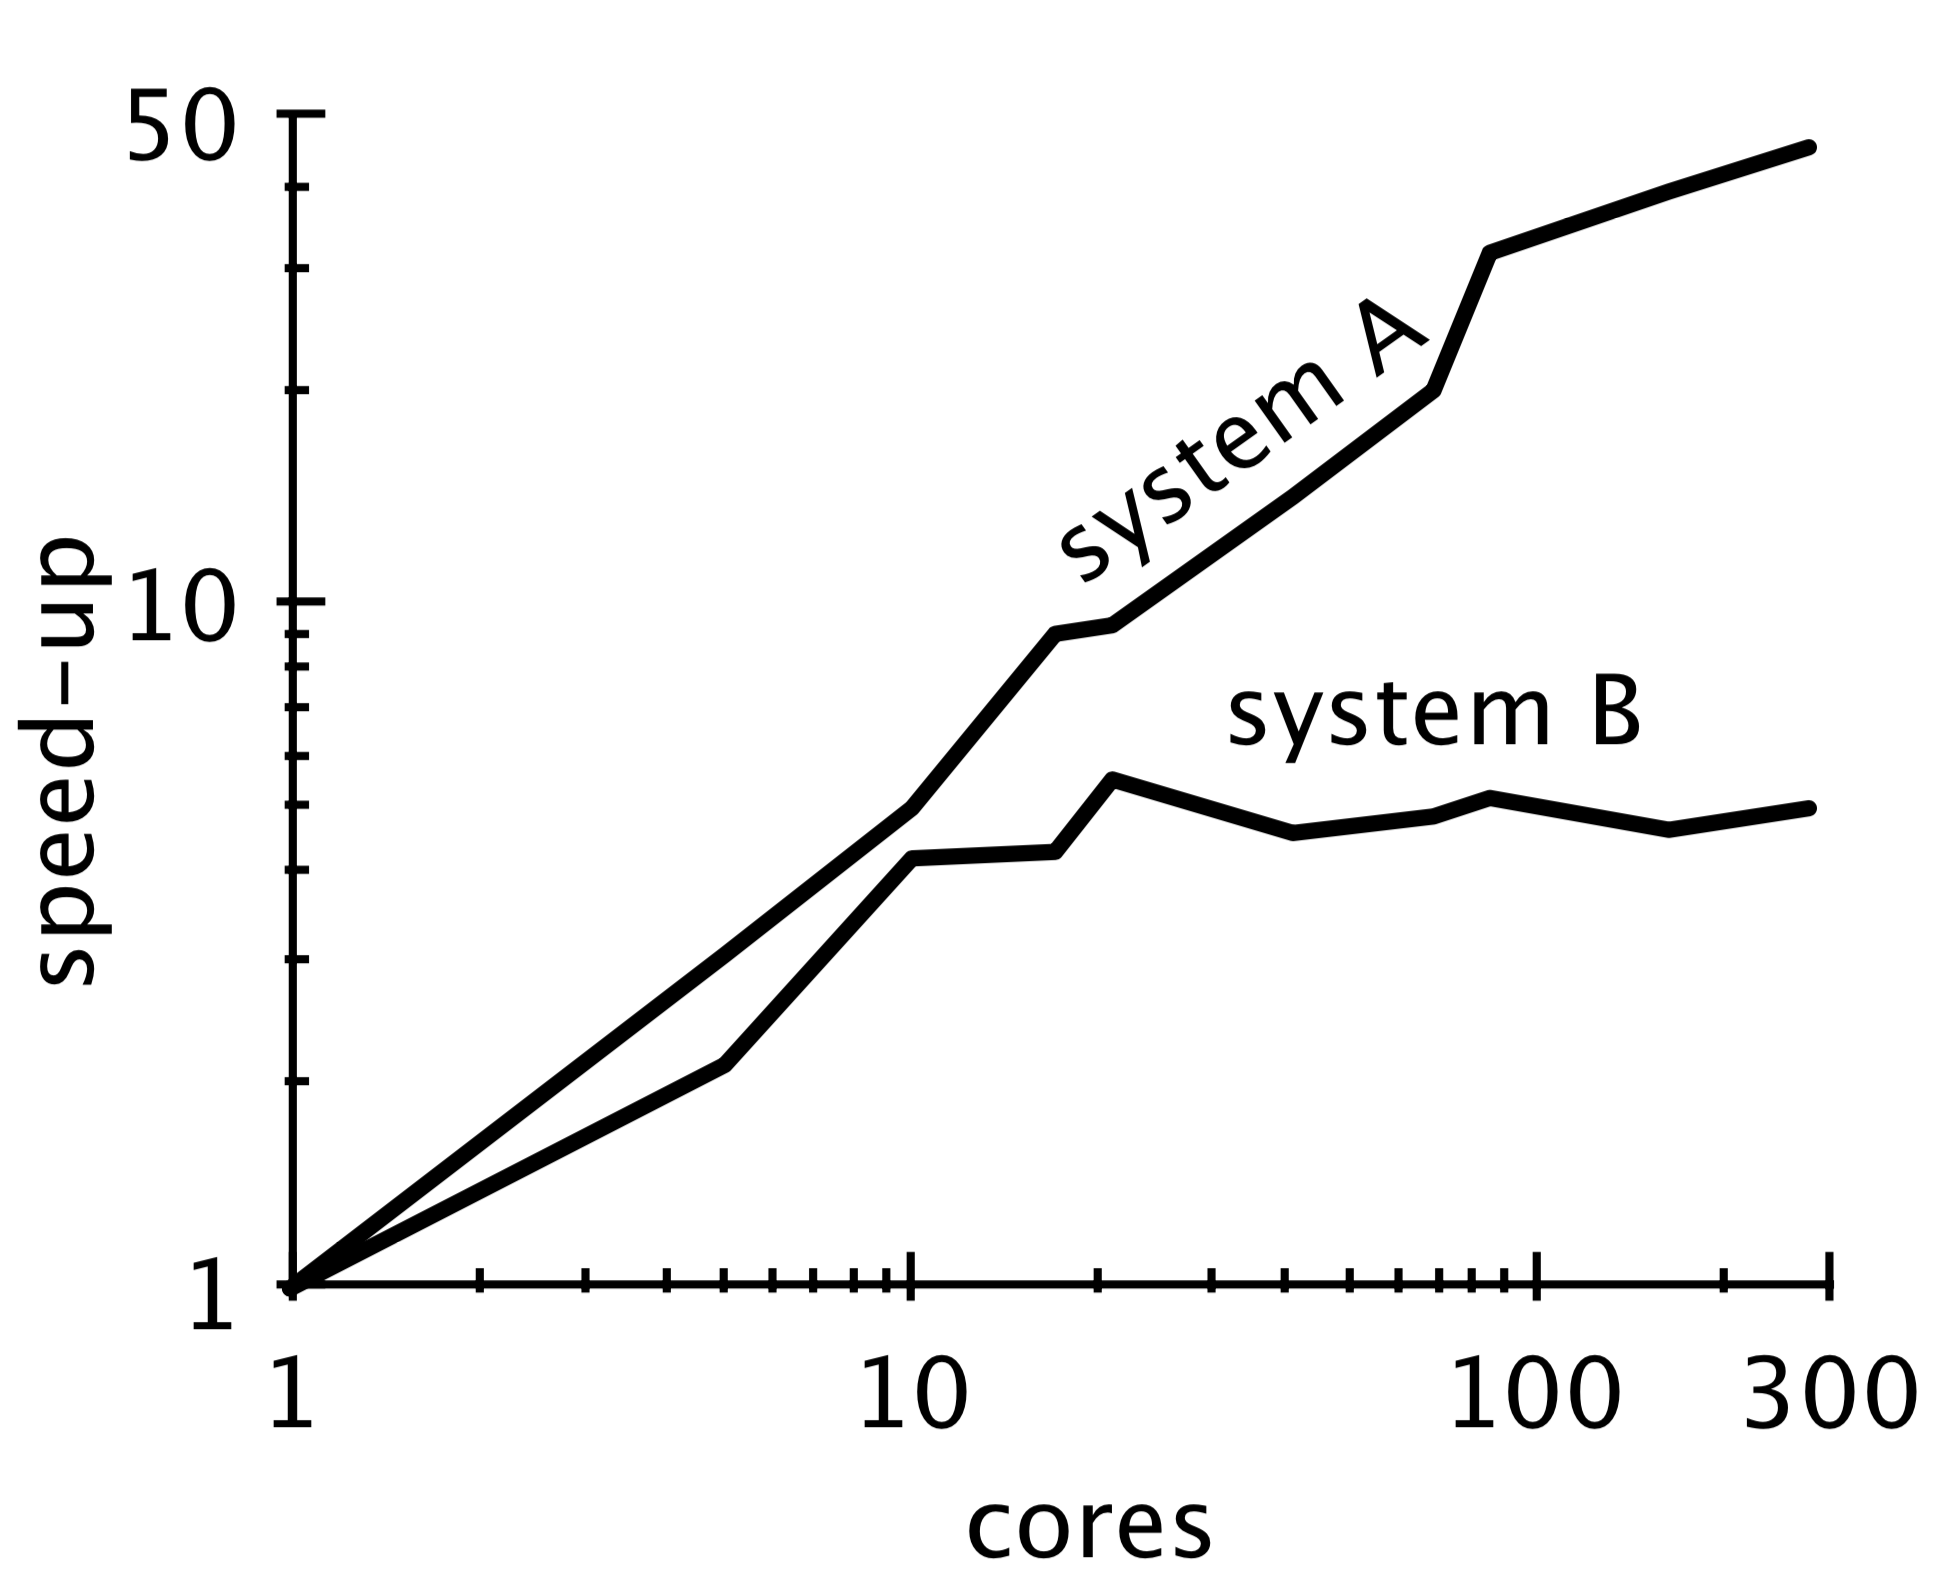
\includegraphics[width=0.76\textwidth]{scalability-1}
  \end{center}
\end{frame}

\begin{frame}[t]{What about now, A or B?}
  \begin{center}
    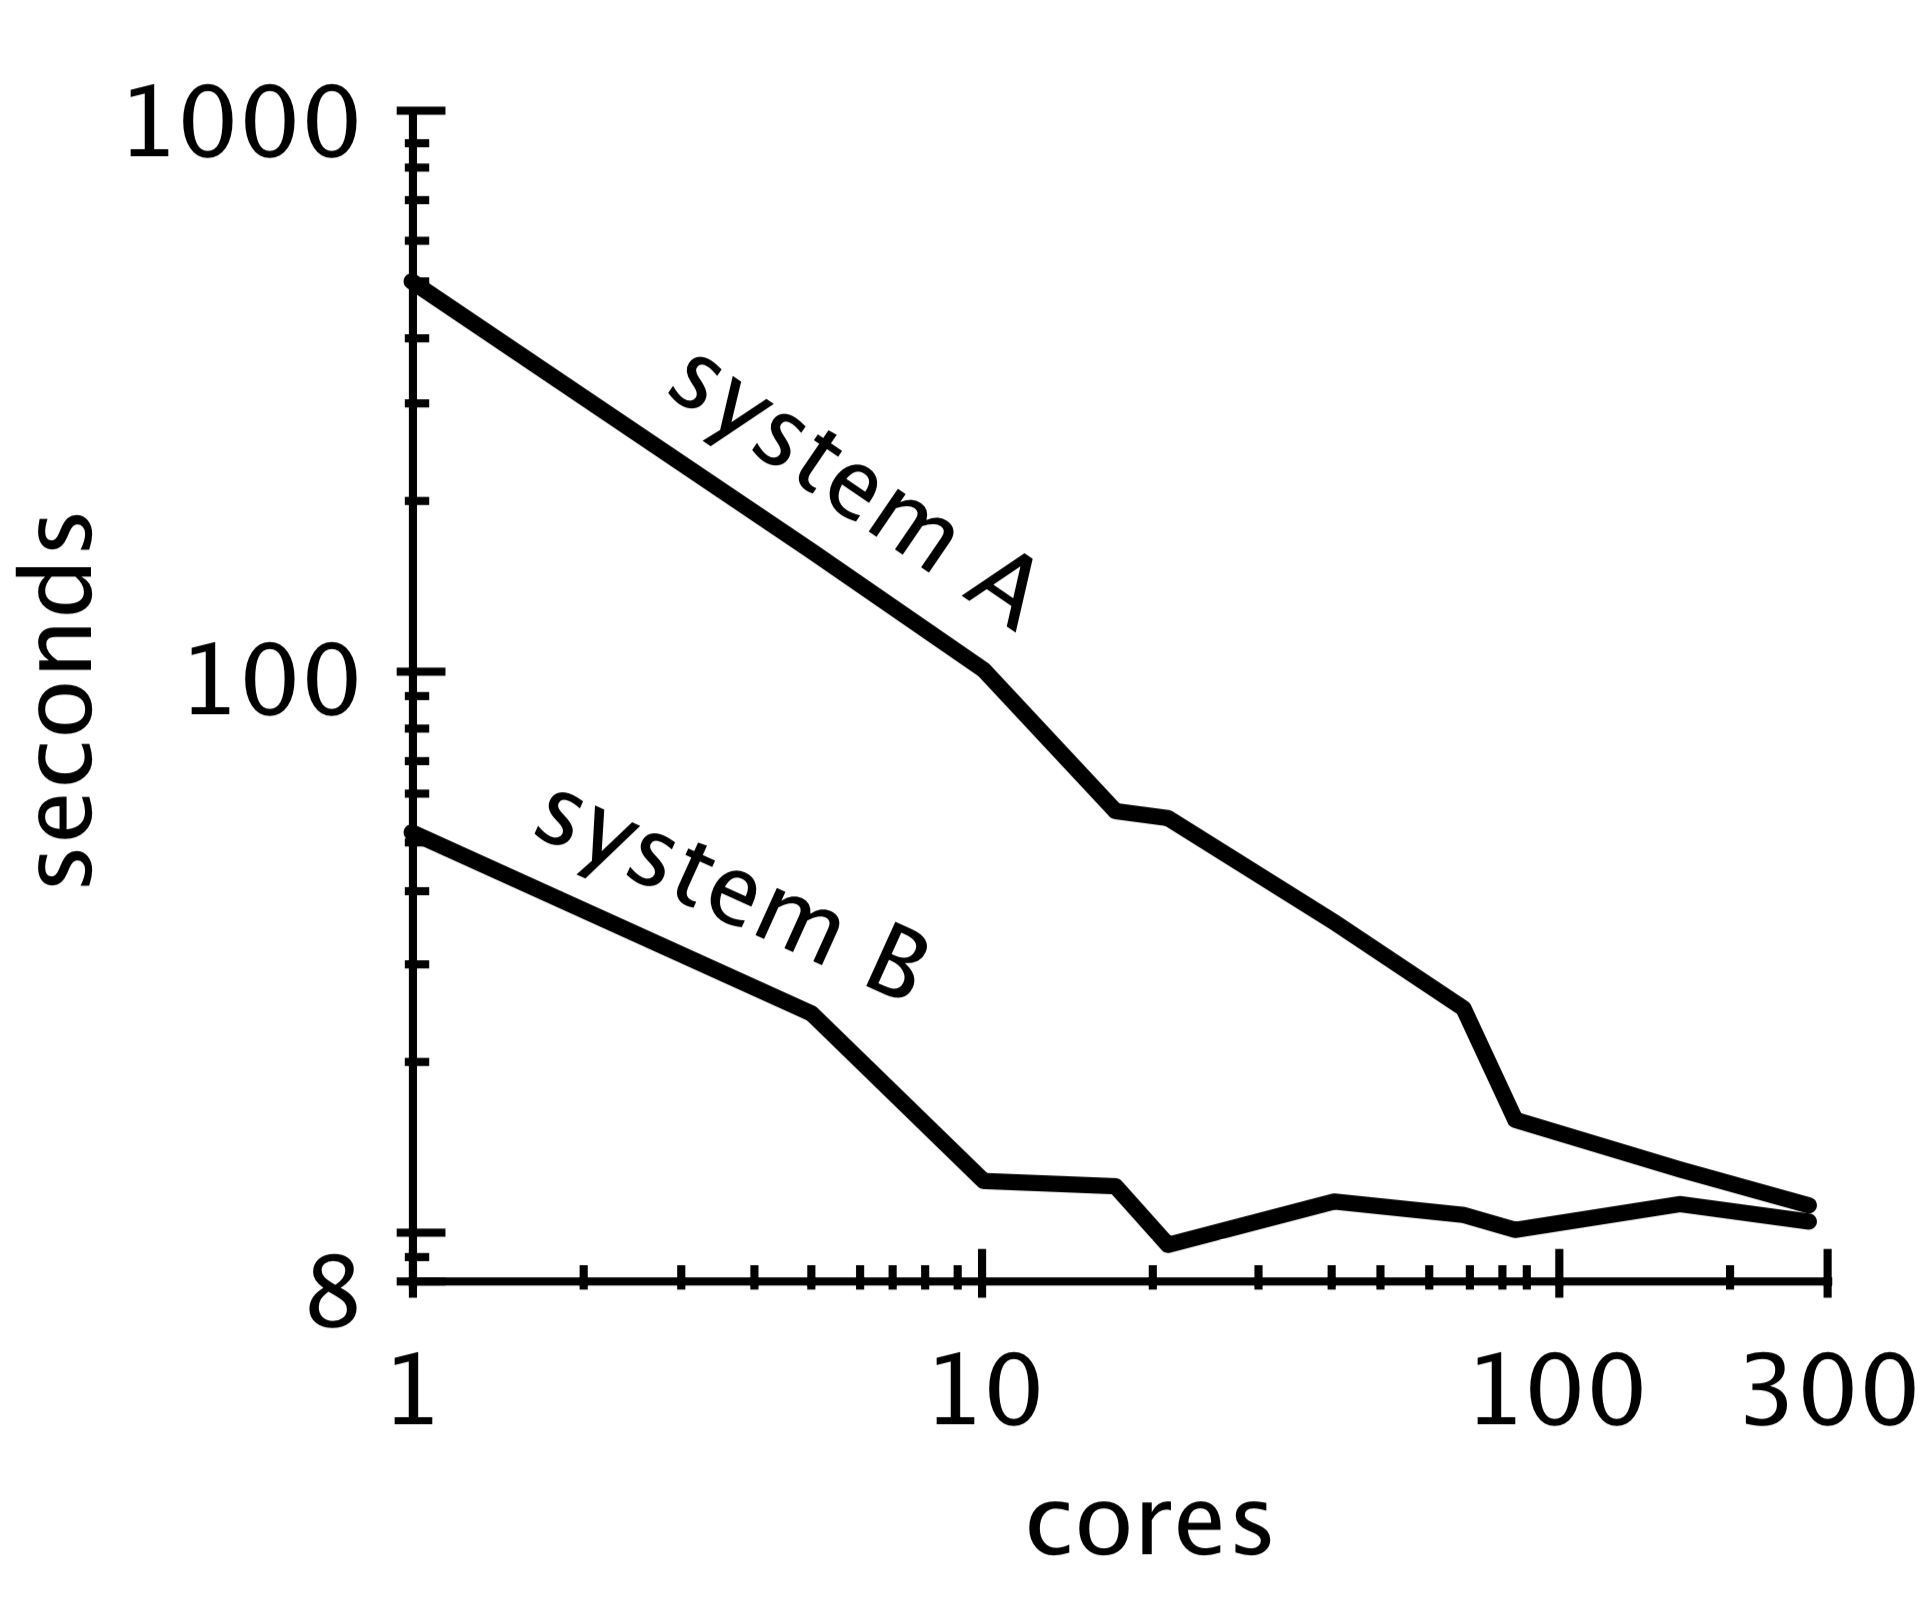
\includegraphics[width=0.76\textwidth]{scalability-2}
  \end{center}
\end{frame}

\begin{frame}[t]{Question in hand}
  \begin{center}
    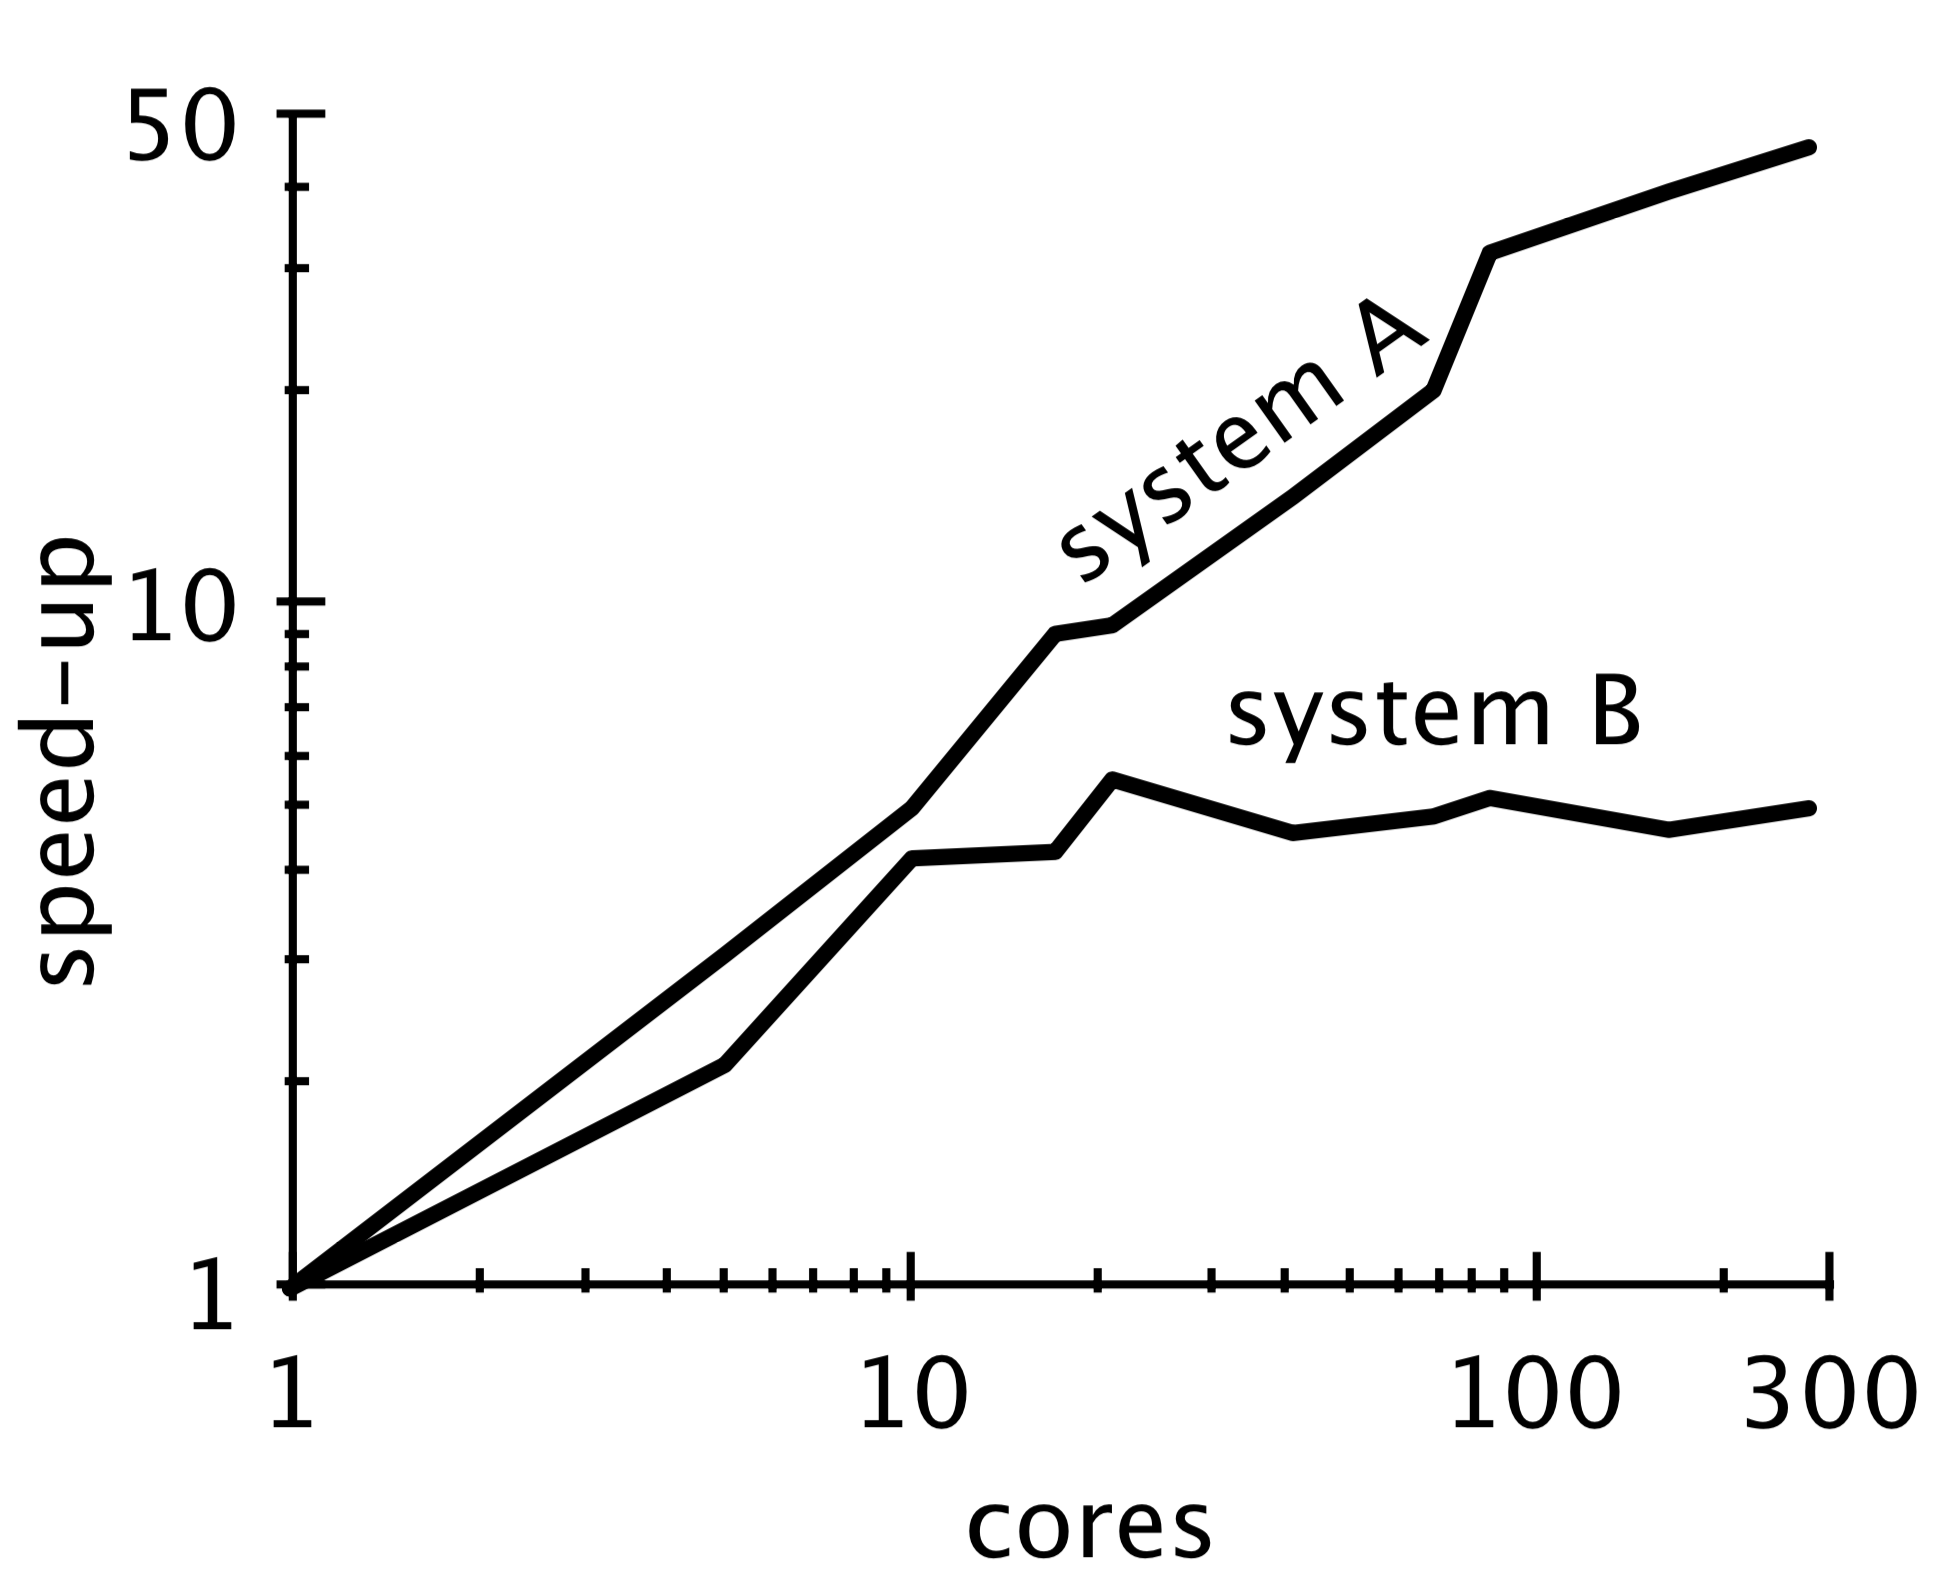
\includegraphics[width=0.42\textwidth]{scalability-1}
    \hspace{0.5cm}
    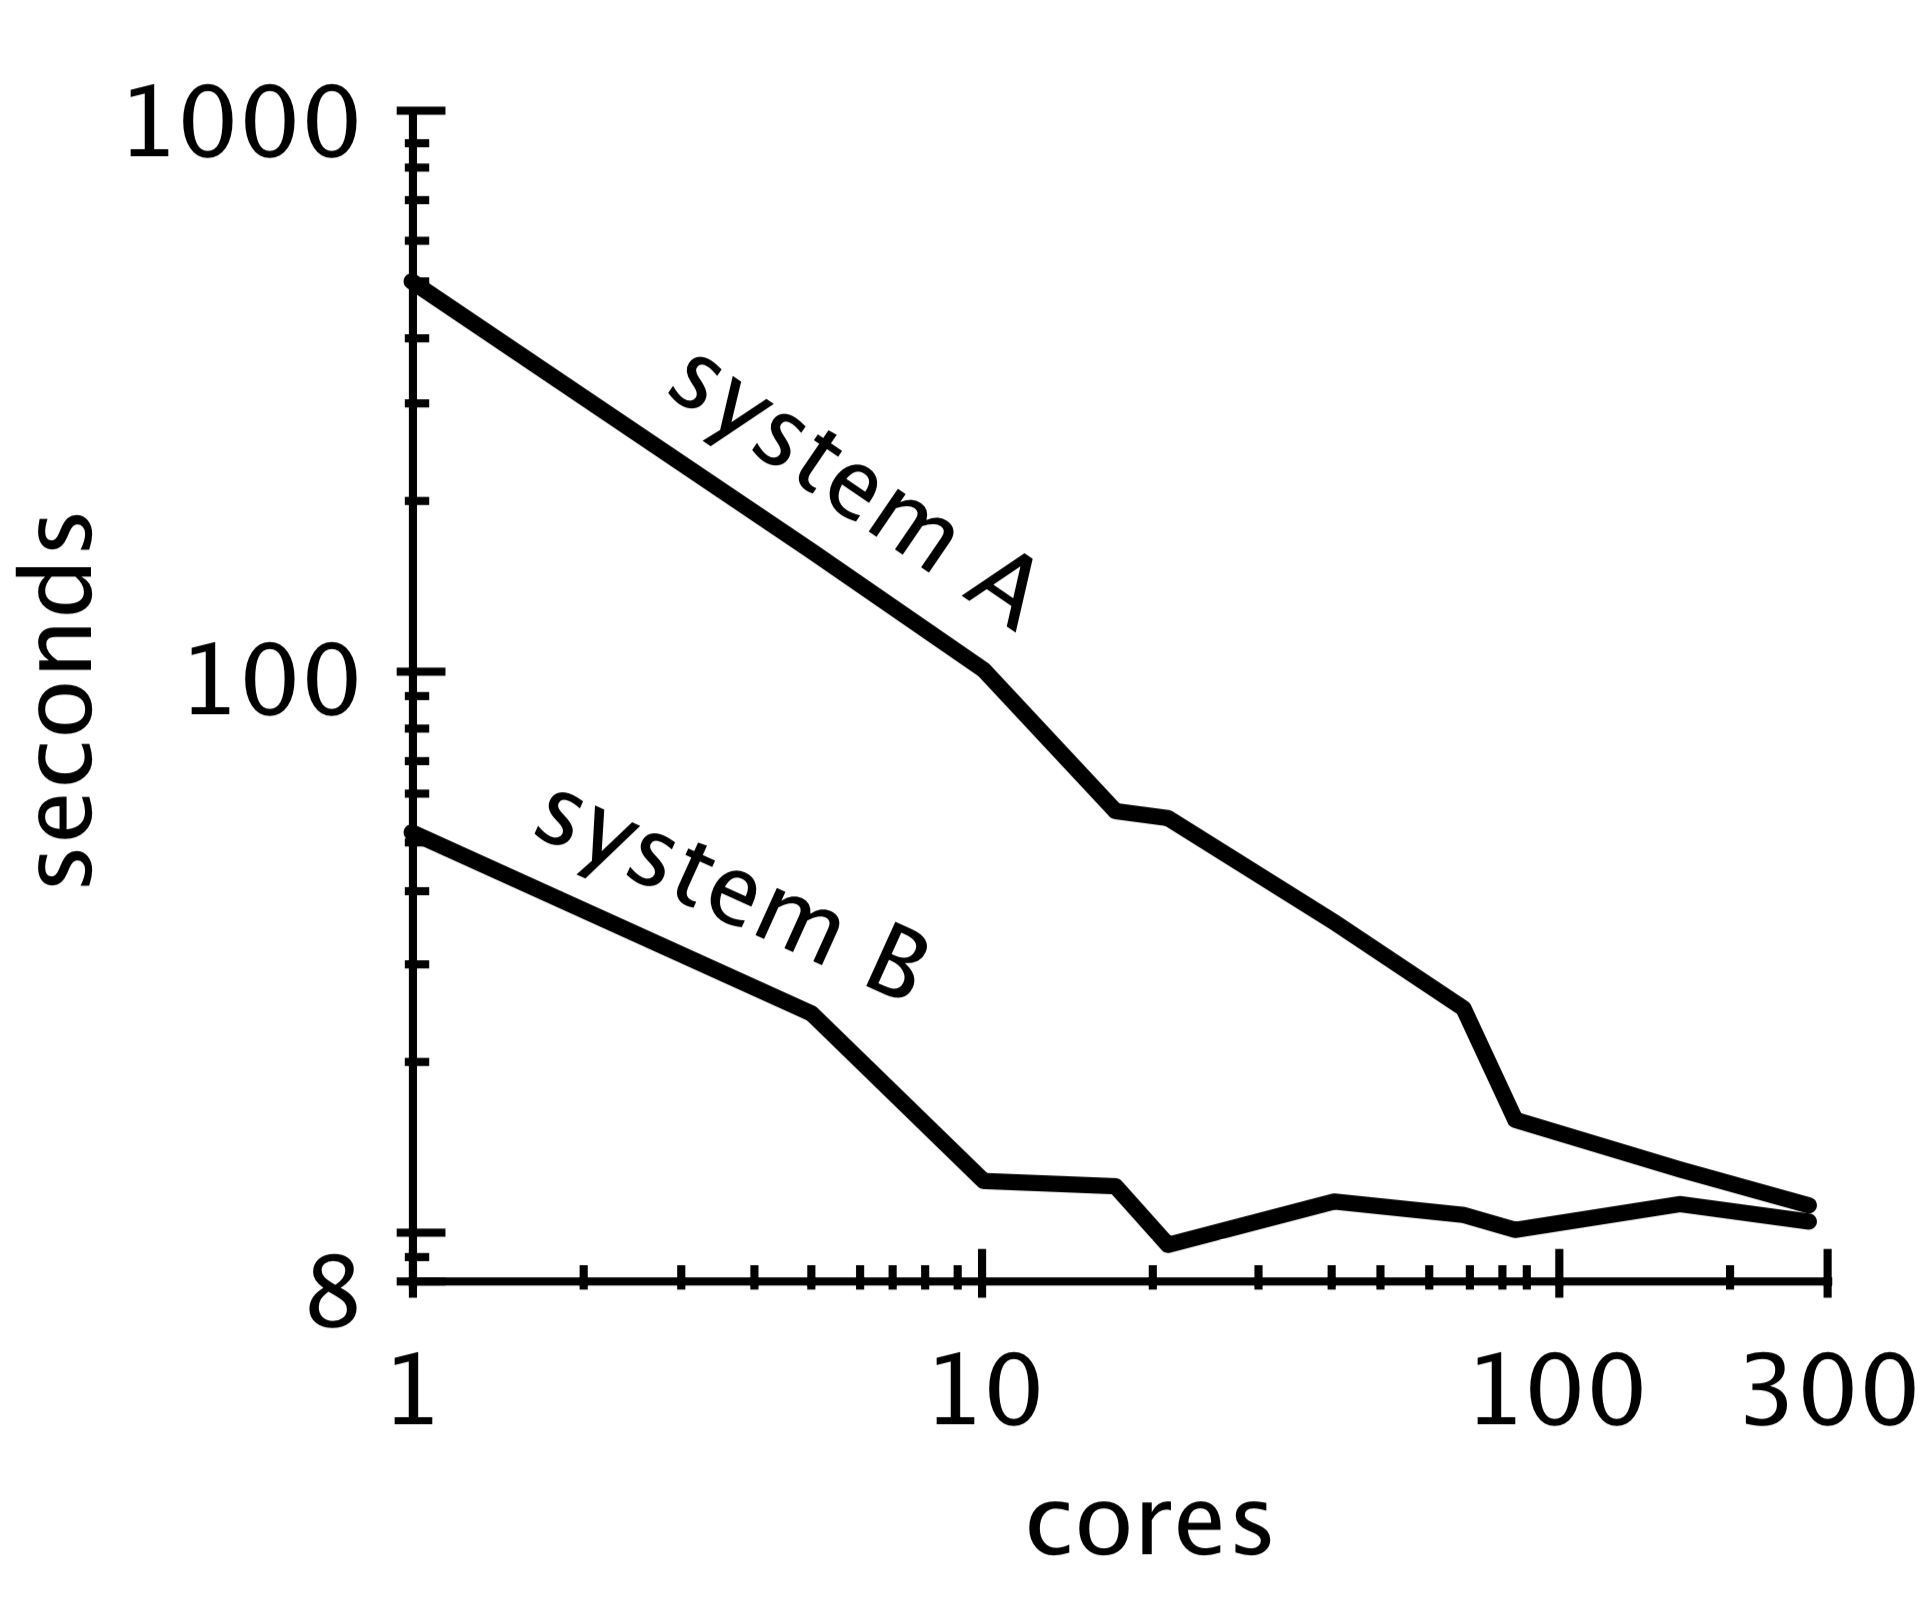
\includegraphics[width=0.42\textwidth]{scalability-2}
  \end{center}

  \begin{itemize}
    \item Scalability is often touted as an essential attribute.
    \item Absolute performance is not related to scalability.
  \end{itemize}

  \vspace{0.5cm}
  \pause

  \textit{To what degree are scalable systems truly improving performance, \\ as opposed to parallelizing overheads introduced?}

\end{frame}

\begin{frame}[t]{How can we measure?}
  \begin{center}
    \Large{"What you can't measure, you can't improve"}
  \end{center}
  \vspace{1.5cm}
  \pause
  COST - \textbf{C}onfiguration that \textbf{O}utperforms a \textbf{S}ingle \textbf{T}hread

  \vspace{1.5cm}
  Why measure against a single thread?
  \begin{itemize}
    \item Distributed systems can have huge overheads.
    \item Most systems have \textit{unbounded} COST!
    \item More optimizations can be applied 
  \end{itemize}
\end{frame}
\begin{frame}[t]{A case study - \textit{Graph} Big Data Systems}

  \vspace{0.5cm}

  Why choose Graph?

  \begin{itemize}
    \item Non-trivial to parallelize
    \item Data-driven
    \item No structure
    \item More time to pass information
  \end{itemize}

  \vspace{0.5cm}

  \pause

  Vertex Centric

  \begin{itemize}
    \item Program from a vertex perspective
    \item Only messages from other vertices as input
    \item Useful for PageRank and other graph algos
    \item "Think Like A Vertex", Pregel, etc.
  \end{itemize}

  \vspace{0.5cm}
\end{frame}

\begin{frame}[t]{PageRank (20 Iterations)}
  \begin{center}
    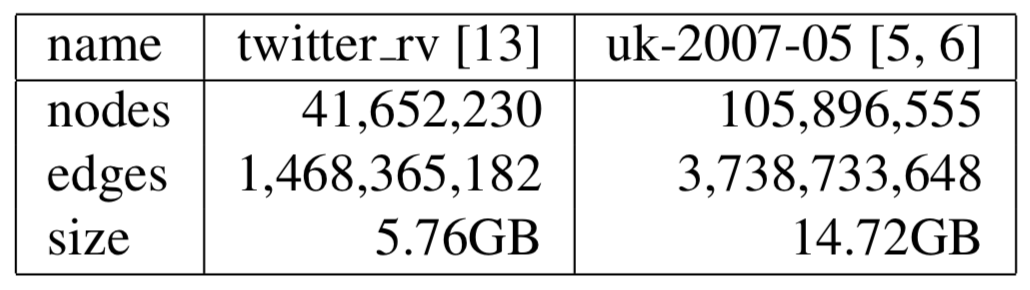
\includegraphics[width=0.65\textwidth]{dataset}
  \end{center}
  
  \vspace{0.5cm}

  \begin{center}
    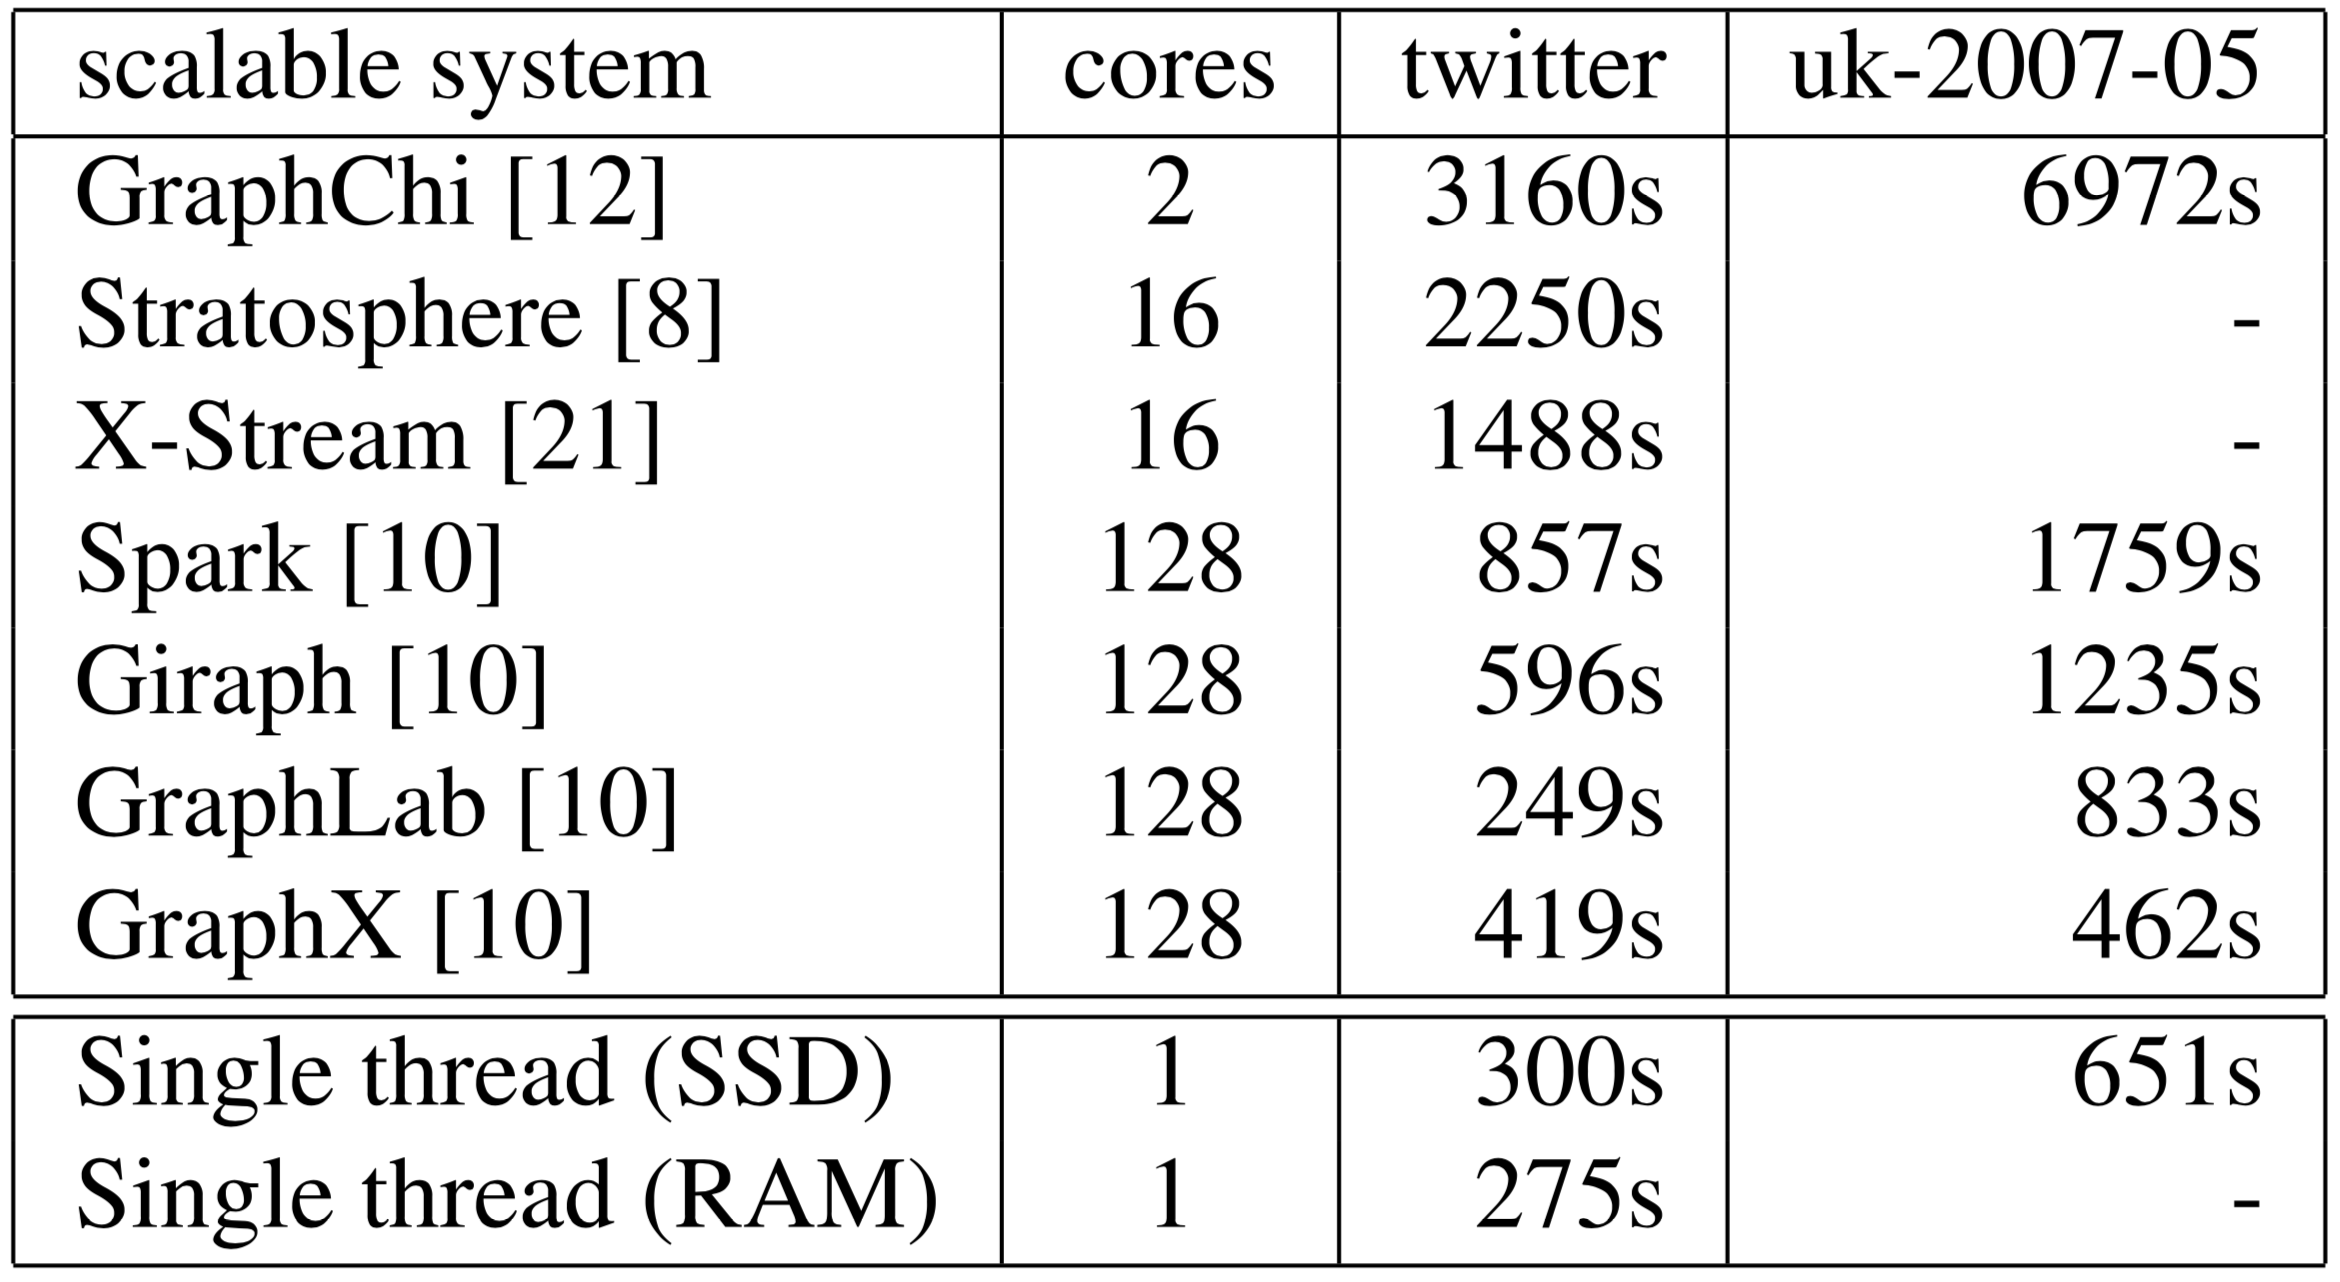
\includegraphics[width=0.75\textwidth]{pagerank}
  \end{center}
\end{frame}

\begin{frame}{Label Propagation (Connected Components)}

  \vspace{0.25cm}

  A common machine learning technique

  \vspace{0.5cm}

  \begin{center}
    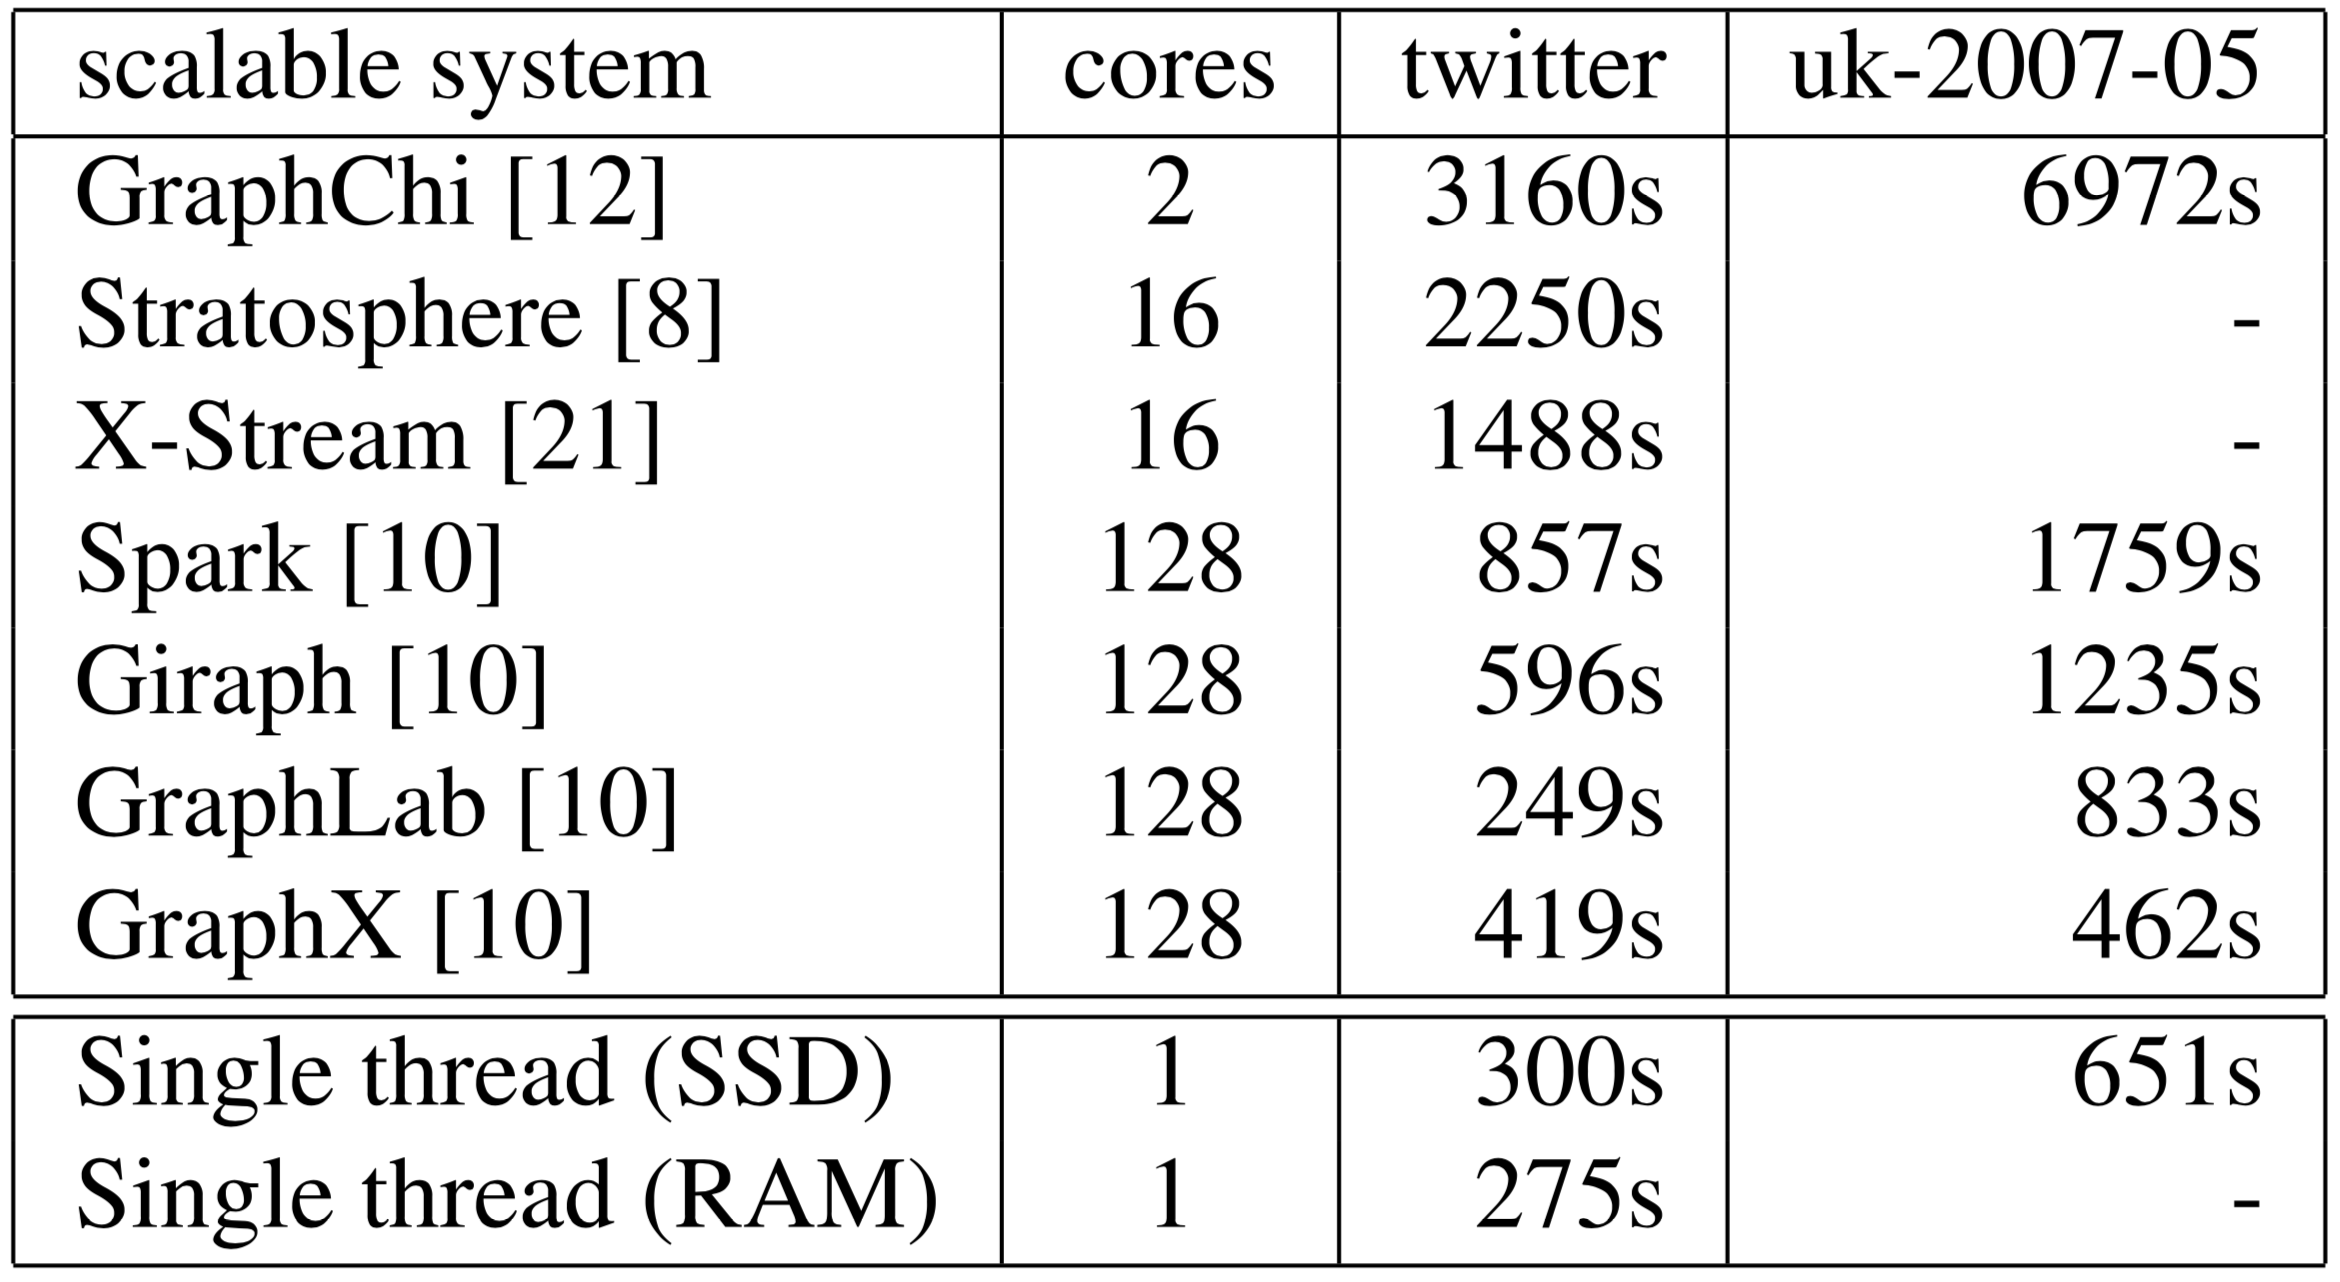
\includegraphics[width=0.75\textwidth]{pagerank}
  \end{center}
\end{frame}
\begin{frame}[t]{More Optimization - Data Layout}
  \begin{itemize}
    \item The order in which edges are presented affects performance.
    \item Hilbert order vs Vertex order.
  \end{itemize}

  \pause

  \vspace{0.25cm}

  Hilbert Curves - Cleverly ordering the edges\footnote{More at https://bigdataatsvc.wordpress.com/2013/07/02/graph-analysis-and-hilbert-space-filling-curves/}
  \begin{itemize}
    \item Assume that edges are stored in an adjacency matrix
    \item Recursively partitions the matrix
    \item Excellent for memory locality + parallelizing
  \end{itemize}

  \begin{center}
    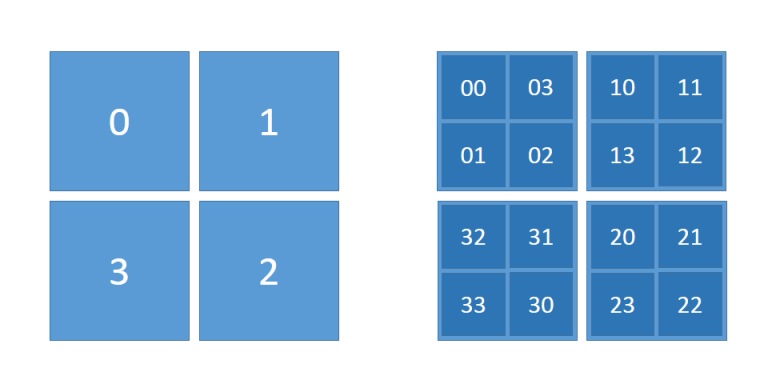
\includegraphics[width=0.65\textwidth]{hilbert}
  \end{center}
\end{frame}

\begin{frame}[t]{More Optimization - Data Layout}
  \begin{itemize}
    \item The order in which edges are presented affects performance.
    \item Hilbert order vs Vertex order.
  \end{itemize}

  \vspace{0.5cm}
  \begin{center}
    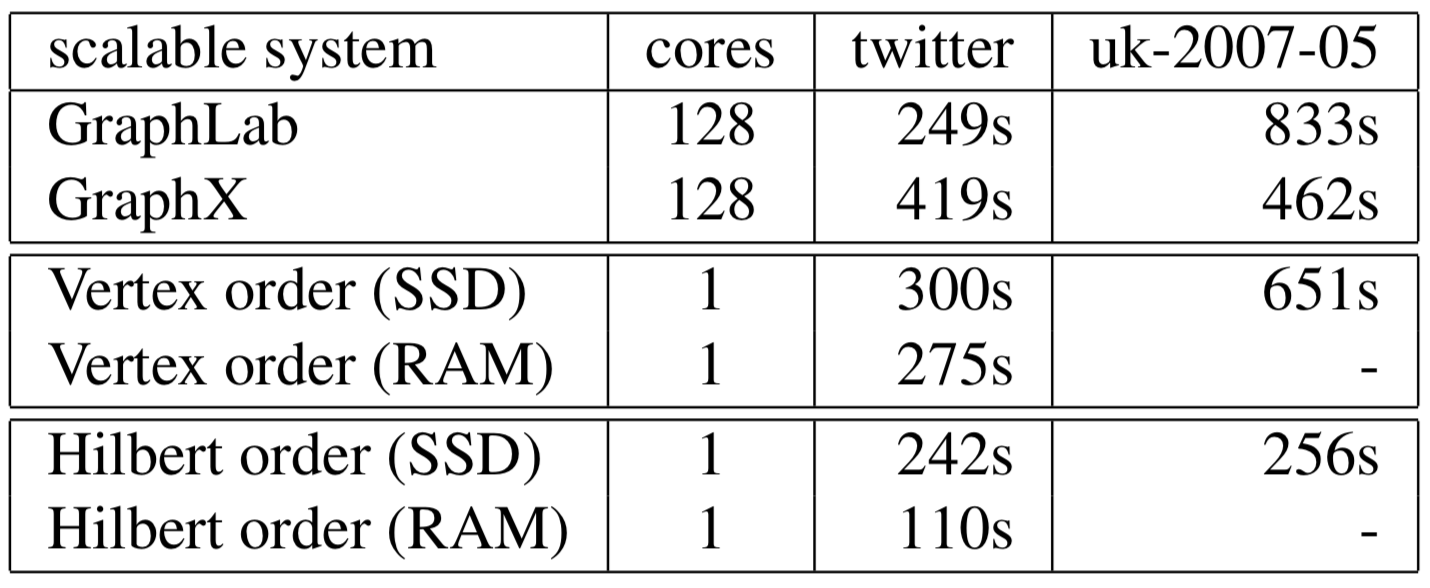
\includegraphics[width=0.75\textwidth]{data-layout}
  \end{center}
\end{frame}

\begin{frame}[t]{Even More Optimization! - Programming Model}
  \begin{itemize}
    \item We are not restricted to "Think like a Vertex" programming model.
    \item Label propagation is sub-optimal, typically $O(n^3 + mn^2)$
    \item Use Weighted Union-Find, $O(m \log{n})$
  \end{itemize}

  \pause

  \vspace{0.5cm}
  \begin{center}
    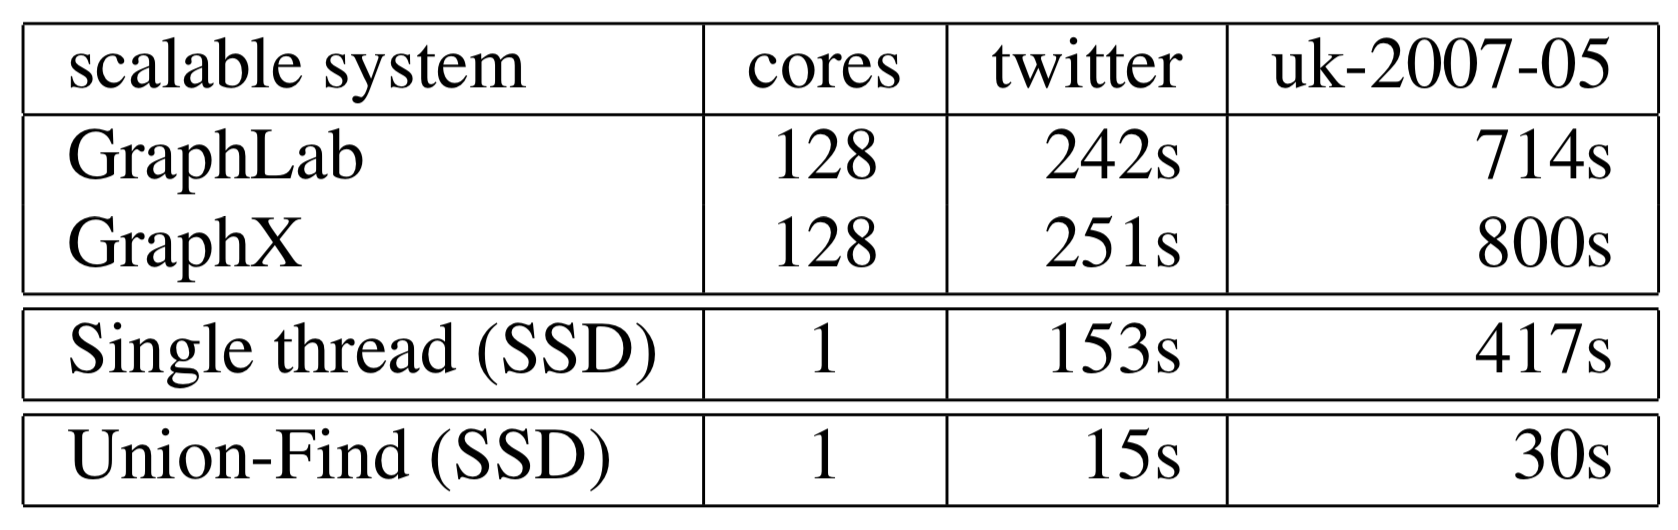
\includegraphics[width=0.75\textwidth]{union-find}
  \end{center}
\end{frame}

\begin{frame}[t]{Applying COST}

  \vspace{0.25cm}

  COST is the point of intersection\footnote{Plots simplified for illustration purposes}

  \begin{center}
    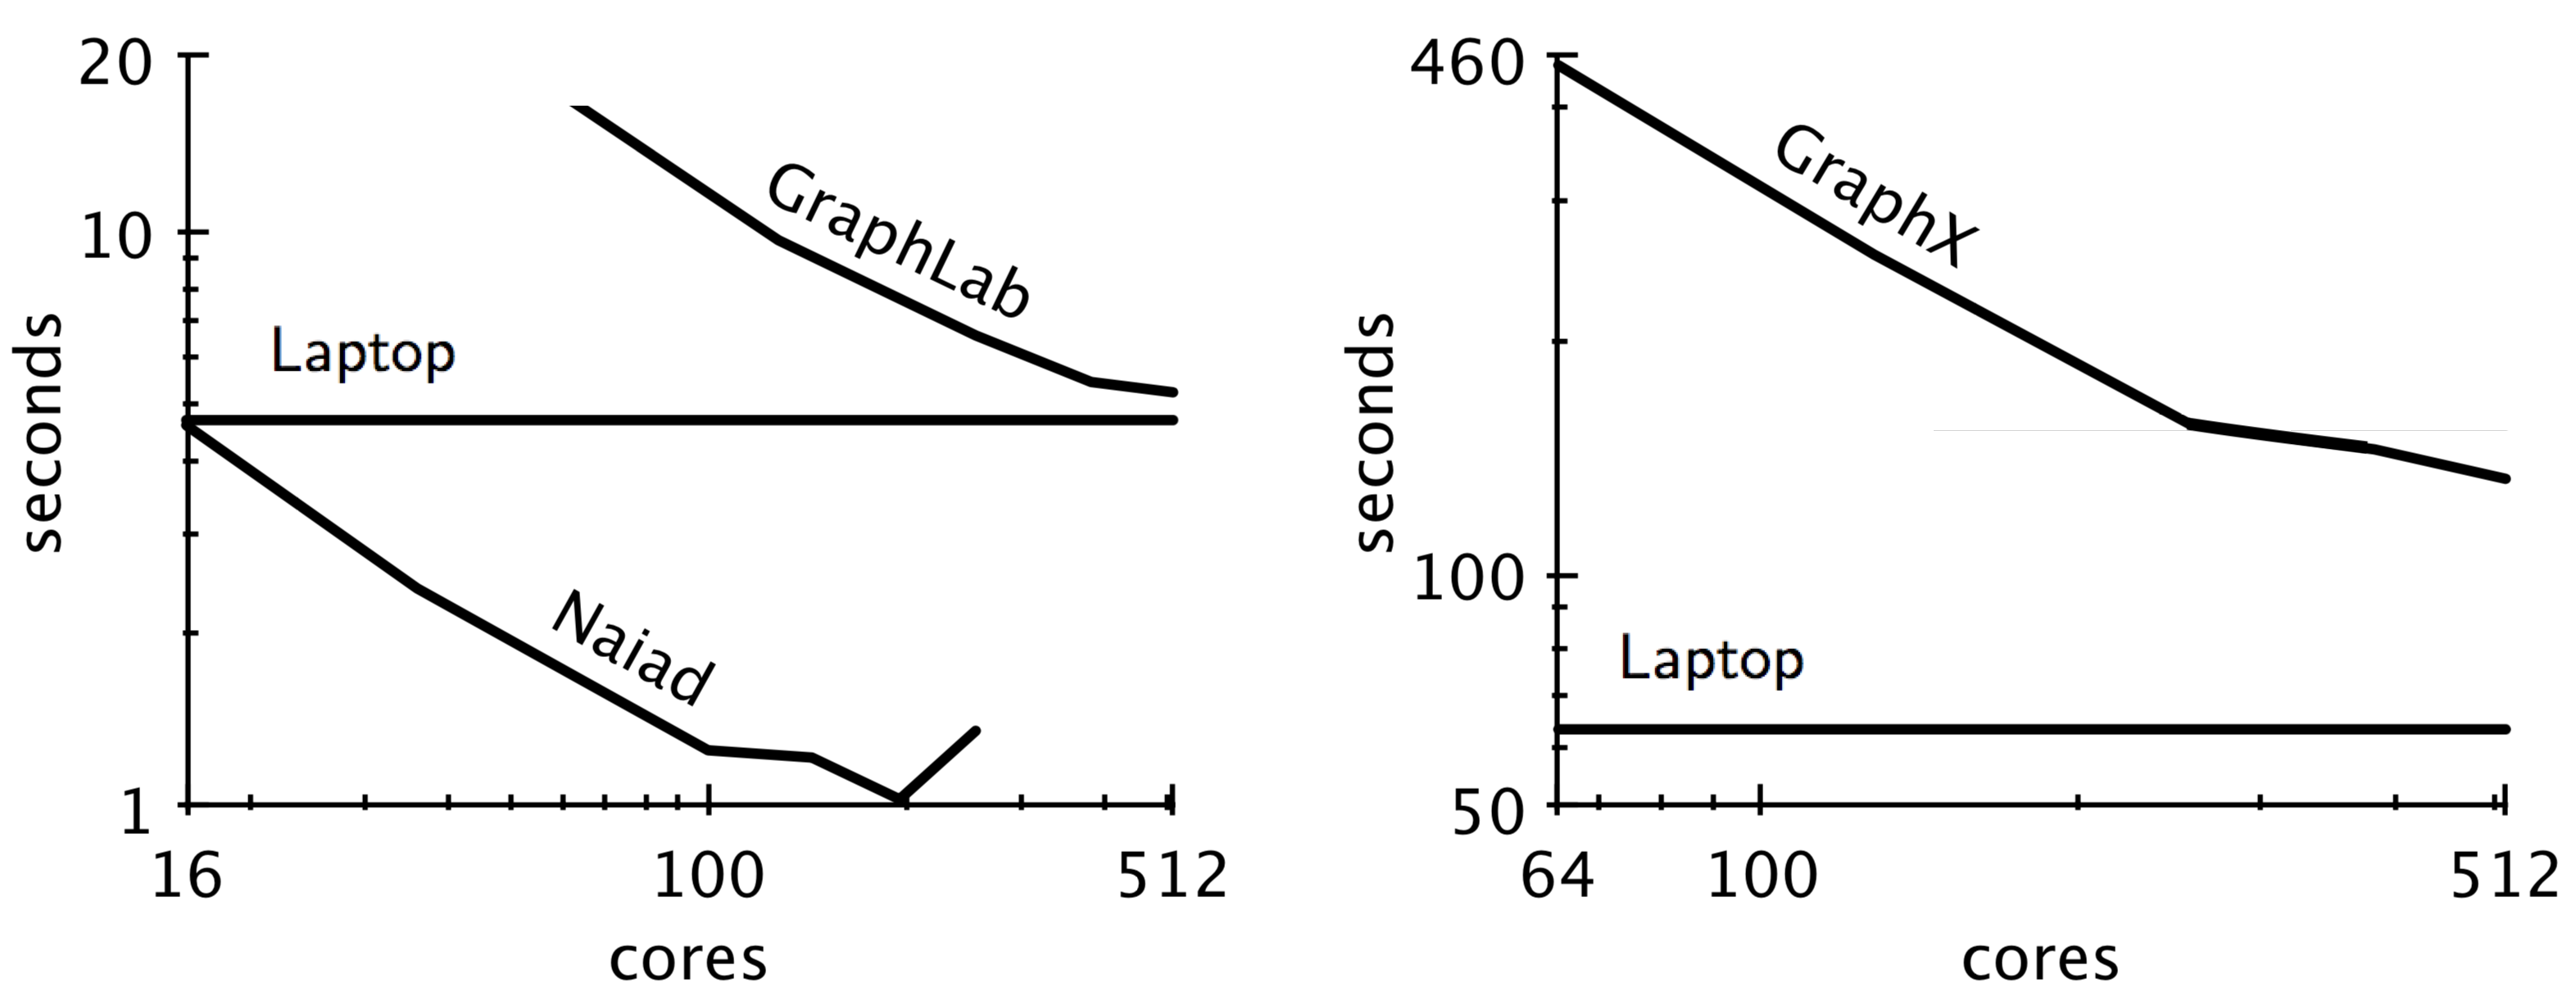
\includegraphics[width=0.95\textwidth]{applying-cost}
  \end{center}

  \pause

  \begin{itemize}
    \item Naiad has a COST of 16 cores for PageRank
    \item GraphX has an unbounded COST (does not intersect)
  \end{itemize}
\end{frame}
\begin{frame}[t]{Lessons}

  \pause

  \begin{center}
    \large{Scalability != Performance}\\
    \vspace{0.1cm}
    \textit{"Can it scale well?"} - not the right question!
  \end{center}
  
  \vspace{0.5cm}
  \pause
  
  Before you build a big data system,
  \vspace{0.1cm}
  \begin{itemize}
    \item Beware of misleading marketing. "One tool for all screws"
    \item Self-investigation is necessary.
    \item Use appropriate algorithms.
    \item Choose to solve the problem locally,\\ don't distribute unless absolutely necessary.
  \end{itemize}

\end{frame}

\begin{frame}[t]{Interesting stuff}

  \vspace{0.25cm}

  Further reading:
  \vspace{0.25cm}
  \begin{itemize}
    \item Boruvka’s algorithm
    \item Galois and Ligra systems
    \item Naiad - timely dataflow
  \end{itemize}

  \vspace{0.5cm}

  People/Things to follow:\\
  \vspace{0.25cm}
  \textbf{Frank McSherry} - https://github.com/frankmcsherry/\\
  \vspace{0.30cm}
  \textbf{Kyle Kingsbury} - https://aphyr.com/\\
  \vspace{0.25cm}
  \textbf{Jepsen} - https://github.com/jepsen-io/jepsen 

\end{frame}

\begin{frame}[t]{Interesting stuff}

  \vspace{0.25cm}

  \begin{center}
    
\includegraphics[width=0.80\textwidth]{debunking}
  \end{center}

\end{frame}




\begin{frame}<handout:0>[noframenumbering]
  \begin{center}
    \huge{Thank you!} \\
    \vspace{1.5cm}
    \large{Questions}
  \end{center}
\end{frame}

\end{document}
